\documentclass[12pt,letterpaper]{article}
\usepackage{anysize}
\usepackage{indentfirst}
\usepackage{sectsty}
\usepackage{amsmath}
\usepackage{hyperref}
\usepackage{graphicx}
\usepackage{caption}
\usepackage{subcaption}
\usepackage{chngpage}
\usepackage{enumerate}
\hypersetup{
	colorlinks=true, 
	linkcolor=blue, 
	urlcolor=blue, 
	pdfnewwindow=true, 
	citecolor=black
}
\urlstyle{same}
\linespread{1.2}


\makeatletter
\renewcommand\@biblabel[1]{\textbf{#1.}} % Change the square brackets for each bibliography item from '[1]' to '1.'
\renewcommand{\@listI}{\itemsep=0pt} % Reduce the space between items in the itemize and enumerate environments and the bibliography


\begin{document}

\begin{titlepage}
    \vspace*{4cm}
    \begin{flushright}
    {\huge
        Quad Control\\[5mm]
    }
    {\large
        CS 472 | Spring 2015
     }
    \end{flushright}
\hrule
    \begin{flushright}
	Audrey Sullivan\\
	Vedanth Narayanan\\
    \vfill
	\today\\
    \end{flushright}
\end{titlepage}

\raggedright

\section*{Introduction}
\hspace{1cm}In an age where we can monitor our cats from our wearables and automatically tweet when we pull on our pajamas, it was a challenge to come up with a unique wearable that serves a new purpose. Wearables can't be mentioned without mentioning smartwatches. Although smartwatches are quite new, we have already seen that they have a wide variety of functionality.\\
\hspace{1cm}We had many wearable ideas that we sifted through, including anklets for activity tracking, wearables that would detect body temperature and modify the room temperature, and perhaps even a wearable for cold-blooded pets. Despite being interesting ideas, they seemed a bit "stale." We wanted to come up with something that could carry on into the future. We started to consider other new tech devices that our wearable could connect to. One thing that popped into our minds was an air drone or a quadcopter. One can buy a quadcopter on Amazon for less than \$50.00. As these are becoming a more popular item, perhaps we could design an innovative wearable to control a quadcopter. This is the concept that we were finally exited to research.

\section*{Concept Design}
\hspace{1cm}We propose an original wearable device that is capable of steering and controlling a quadcopter. It would be very convenient to be able to direct a droid with a wristband-like device, with vertical and horizontal directing controls. This device would simplify control functionality and be a great alternative to large handheld controllers.\\
\hspace{1cm}Our design utilizes an obtuse isosceles triangular shape that allows you to control with your index finger and thumb, representing the X-Y plane, and Z dimension. Since thumbs are less mobile, they would control strictly Z while the index finger can operate the X-Y plane. Where the top face represents X-Y plane and the bottom face acts in the Z (upward and downward) dimension. You can essentially use two wide sides of a triangle with the obtuse angle on top to control different directions at the same time while the third face is attached to the wristband. Prototype design is focused on later on in the report.\\
\hspace{1cm}We plan to keep all of the essential power and microcontroller housed inside of the pyramid-like structure. The main components of our device include two batteries, a microcontroller, and touch sensors.\\
\hspace{1cm}Our idea is to send the copter commands to an app, and have the app send the commands to the quadcopter. Some of the apps that exist today include Quadroid for Android and Astrodrone for Android/iOS. \\
\hspace{1cm}Students at MIT have created a wearable device called NailO, which allows you to control devices from your nail space. The device works by sticking it to a nail (usually thumb) like you would a nail sticker and use another finger on that hand to drag on that surface. We are using similar principles in our design to obtain two NailO like pads on the two faces of the triangular design. \\

\subsection*{Assumptions}
\begin{itemize}
\item Assume the app communicating with our device has secure features such as a secure bluetooth connection that stops other apps from controlling the same quadcopter. 
\item The device, unlike conventional wearables, will not always be on. It’s meant to only be turned on when it needs to be used. 
\item To be able to properly piggyback on an existing  mobile application, there are definitely changes that need to be made, including being able to connect to the device through Bluetooth, and properly parsing the commands from the device, and then passing them off to the quad copter.
\item NailO has its own microcontroller that we want to strip out and connect the touch sensors to our microcontroller.
\item NailO doesn't mention the type of touch sensors that were used, but we are going to assume it is Atmel AT42QT2640 Touch controller.
\end{itemize}

\subsection*{Use Cases}
\begin{itemize}
\item I want to be able to integrate Quad Control with my Quadroid App.
	\begin{itemize}
		\item Our assumptions are that you can use Quad Control as a accessory to an existing smart phone app.
		\item We will have room for extra capabilities in case more wants to be added to the Quad Control if the app has further functionality than steering.
	\end{itemize}
\item I want to be able to click to change settings from Quad Control.
	\begin{itemize}
		\item You can use the touch pads as buttons with a tap.
	\end{itemize}
\end{itemize}

\subsection*{Prototype}
\hspace{1cm}The design we propose may look simple, however it did not come about this way without purpose or thought. The general design idea was primarily dependent on the items we wanted to place in the device. Clearly, having a huge processor and the biggest batteries and sensors was challenging to fit in a sleek wearable design.\\

\begin{figure}
	\centering
	\begin{subfigure}{.5\textwidth}
		\centering
		\includegraphics[width=1\linewidth]{CaptureV1.png}
		%\caption{A subfigure}
		\label{fig:sub1}
	\end{subfigure}%
	\begin{subfigure}{.5\textwidth}
		\centering
		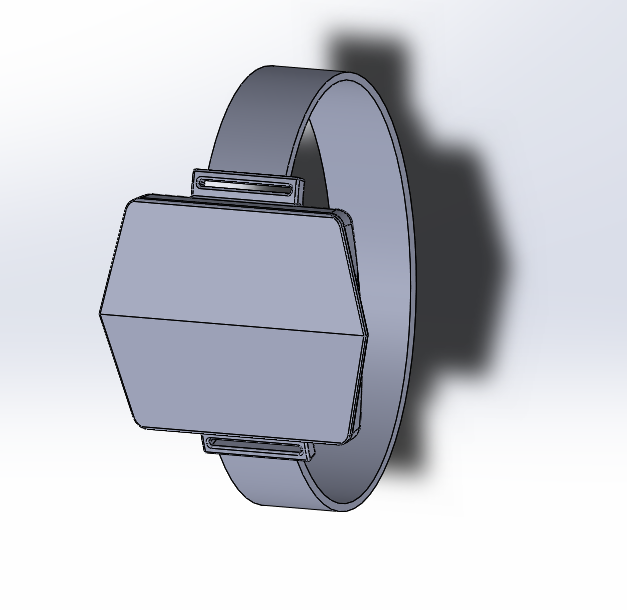
\includegraphics[width=1\linewidth]{CaptureV5.png}
		%\caption{A subfigure}
		\label{fig:sub2}
	\end{subfigure}
	\caption{The overall design of the Quad Control wearable device.}
	\label{fig:test}
\end{figure}

\hspace{1cm}We were initially looking into having a small processor like the new Intel Curie or something from the AMD Cortex M series, but remembered from ECE 375 that we don't always need a processor. More often than not a microcontroller will do, and a processor will only hike the device price. Thus, we went on to look for microcontrollers that would service our needs. We found the "Adafruit GEMMA v2" microcontroller that was circular in shape, and we decided to design around that.\\
\hspace{1cm}We then continued to look for track pads and batteries that would go along with the microcontroller that we had chosen. Very soon, we found out about NailO, an MIT research project, which was on a similar path to the one we were following. We realized that we could use the touch sensors that they were using for our device. Once again on the Adafruit website we found a battery that could be used. Once we had what we thought we might need, we consulted one of our Mechanical Engineering friends, Caleb Schmidt, to discuss whether building a device like this would be possible and mock up a design on Solidworks for us.\\

\hspace{1cm}Talking to Caleb was really useful for us because he gave us a general sense of the thickness of our device, if we were to place all the materials we had gathered in there. After much debate, he helped us come with a design that could potentially work, if we could change a couple of different materials inside.\\
\hspace{1cm}We ended up finding "Bluetooth LE (BLE) Beetle Wearable Microcontroller." We thought this would a better option because the shape was more of a rectangle, Bluetooth was included, and it was wireless programming capable. The drawback was that it needed 5V power, but we were only able to supply 3.7V. We decided to look into Samsung's new wearable batteries. More specifically they had thin curved battery cells that we wanted to use. Originally, the idea was to place them in the wrist strap and save space on top. Instead, a better solution was to elevate the middle of the device into a peak, and place the batteries under the track pad sensors. While we had thought about being able to pop the top of the device off to connect the microcontroller and program it, with the new microcontroller we could wirelessly program it. The design is quite simple because we want the user to not have any problem controlling their copter. Often, you see huge remote controllers that have a variety of knobs and buttons, and the user needs a tutorial before they can fly it. Our device is simple and allows the user to do exactly what they want to.\\
Once we had everything in place, Caleb modeled it for us. Refer to Figures 1 and 2 to get an idea of what it will look like.


\begin{figure}
	\centering
	\begin{subfigure}{.5\textwidth}
		\centering
		\includegraphics[width=1\linewidth]{CaptureV2.png}
		%\caption{A subfigure}
		\label{fig:sub1}
	\end{subfigure}%
	\begin{subfigure}{.5\textwidth}
		\centering
		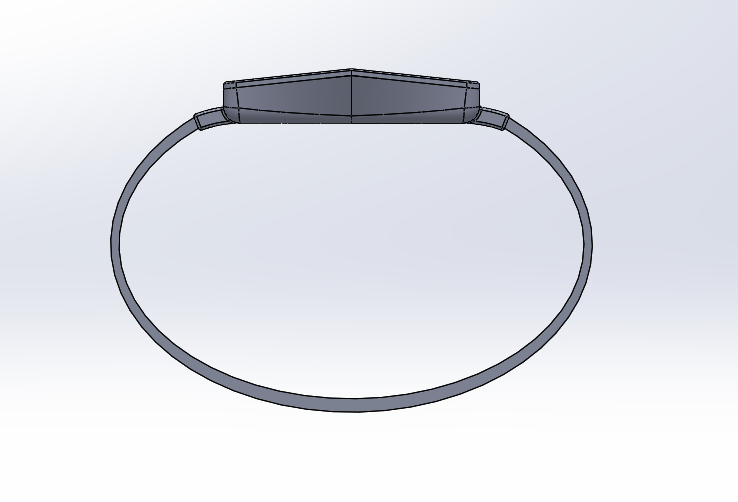
\includegraphics[width=1\linewidth]{CaptureV3.png}
		%\caption{A subfigure}
		\label{fig:sub2}
	\end{subfigure}
	\caption{The device from different angles.}
	\label{fig:test}
\end{figure}

\section*{Specifications}
\begin{tabular}{| l | l |}
	 \hline
	 & Details \\ \hline
	Height &  \\ %\hline
	Length &  \\ %\hline
	Width &  \\ %\hline
	Weight &  \\ %\hline
	Battery Capacity &  \\ %\hline
	Battery Power &  \\ %\hline
	Duration &  \\ \hline
\end{tabular} \\

\subsection*{Pros and Cons}
\paragraph{Pros}
\begin{itemize}
	\item Sleek designed device that is easy to carry.
	\item Simple design, so the user is not confused.
	\item The design is dynamic and more capabilities can be added in the future.
	\item Unlike other wearables, this will not always be turned on.
	\item Battery capacity is 210 mAh, so they will be able to last for a long amounts of time. It would definitely suffice for the amount of time you would need for quadcopter activity. The device will need to also get charged less often.
	\item The microcontroller can be wirelessly programmed.
	\item Bringing James Bond style to real life.
\end{itemize}

\paragraph{Cons}
\begin{itemize}
	\item Quadcopters already have controllers with them, and this is just another device that needs to be carried around.
	\item Microcontroller requires 5V of battery, but we essentially have 7.6V, so this is overkill.
	\item If user has a smart watch, then this is just something else they need to wear.
	\item User needs to own a smartphone to use this.
\end{itemize}

\subsection*{Costs}
\begin{tabular}{| l | l | l |}
	\hline
	Component & Quantity & Total Cost(\$) \\ \hline
	Bluetooth LE (BLE) Beetle Wearable Microcontroller & 1 & 15.28 \\ \hline
	Samsung curved cell (PCF441435) & 2 & $\approx$40.00\\ \hline
	Atmel AT42QT2640 Touch controller & 2 & 18.00\\ \hline
	\textbf{Total} & \textbf{5} & \textbf{73.28}\\ \hline
\end{tabular} \\



\section*{Conclusion}
The Quad Control wearable device that we propose may have little significance now, but will acquire more in the very near future. At the least, quadcopter enthusiasts will have a sleek and simplistic addition to their collection of quadcopter accessories. 

\newpage
\nocite{*}
\bibliographystyle{annotate}
\bibliography{bib}

\end{document}
